\section{Analysis of the motorised antenna stand}\label{sec:AnalysisMotorisedStand}
To be able to efficiently transfer power to a flying done, the stand must be precisely controlled in the azimuth and elevation planes. This way the stand can point in any direction represented by the angle in the azimuth plane $\phi$ and an elevation angle $\theta$, as shown in figure \autoref{fig:laserPointingModel}.
\begin{figure}[h!]
\centering
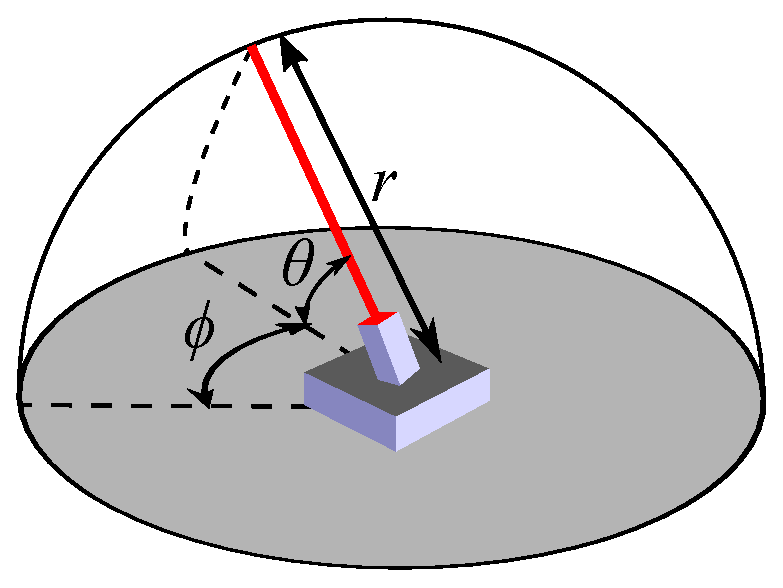
\includegraphics[width=0.5\textwidth]{figures/technical/antennaStandModel}
\caption{Illustration of a laser directed at a point represented by a distance, $r$, angle in the azimuth plane, $\phi$, and an elevation angle, $\theta$.}\label{fig:laserPointingModel}
\end{figure}

The pointing of the antenna stand must be automated and precise for efficient wireless charging of the drone. Therefore the antenna stand must be equipped with motors to allow automatic adjustment in the azimuth and elevation planes through an electrical system. This can be accomplished in different ways, but motors attached to a mechanical construction with low moment of inertia, low dampening and no spring effect constants is desired. The motors should have a low internal resistance, inductance and capacitance and as high a motor torque constant as possible. This would allow for fast and efficient movement along the azimuth and elevation planes. The design of such a system is not covered in this project since a functioning motorised antenna stand has been provided by Aalborg University, as stated in \autoref{ch:TechnicalKnowlegde}. The provided antenna stand is therefore analysed in order to create an effective control system for the stand.

A picture of the provided motorised antenna stand is seen on \autoref{fig:antenna_stand}. The stand includes two motors, a DC motor for moving the azimuth angle and a stepper motor for moving the elevation angle.
\begin{figure}[h!]
	\centering
	\includegraphics[width=\textwidth]{figures/technical/stand}
	\caption{Picture of the motorised antenna stand. The stepper motor and DC motor with their respective gearing is marked. The azimuth, $\phi$, and elevation, $\theta$ planes are also marked.}
	\label{fig:antenna_stand}
\end{figure}

\newpage
To control this system effectively, a model of the mechanical systems and the motors must be developed.
A model is created in three steps.
\begin{enumerate}
\item Determining the mechanical and electrical constants of the DC motor
\item Determining the mechanical constants of the gearing system between DC motor and stands azimuth rotational body.
\item Determining of mechanical and electrical constants of the Stepper motor.
\end{enumerate}
\subsection{Modelling of the DC motor}\label{sec:DC-motorTechnicalKnowledge}
A model of a DC motor can be split into an electrical and a mechanical part, as illustrated on \autoref{fig:DC-motorElecRep} and \autoref{fig:DC-motorMechRep}. 
\begin{figure}[h!]
    \centering
    \begin{subfigure}[b]{0.45\textwidth}
        \includegraphics[width=\textwidth]{figures/design/electrical_model_motor.pdf}
		\caption{Electrical model of a DC motor with a voltage source, $V_s$, attatched.}
		\label{fig:DC-motorElecRep}
    \end{subfigure}
    ~ 
    \begin{subfigure}[b]{0.45\textwidth}
       \includegraphics[width=\textwidth]{figures/design/mech_model_motor2.pdf}
		\caption{Mechanical model of a DC motor with a torque, $\tau_m$, and load, $\tau_l$ applied.}
		\label{fig:DC-motorMechRep}
    \end{subfigure}
    \caption{Illustrations of models of the electrical and mechanical parts of a DC motor \citep{ModelingAndAnalisys} (Variable names modified from original.).}\label{fig:DCMotorModel}
\end{figure}

Two differential equations are developed.  \autoref{eq:DC-motorMechEq} is derived from the freebody diagram of the motor seen on \autoref{fig:DC-motorMechRep}, while \autoref{eq:DC-motorElecEq} is Kirchhoff's voltage law for the electrical representation from \autoref{fig:DC-motorElecRep}. 
\begin{equation} 
v_{s}(t) = R_{a}\cdot i_a(t) + \frac{d i_a(t)}{d t}\cdot L_a + K_{e}\cdot\omega_{m}(t) \addunit{\volt} \label{eq:DC-motorElecEq}
\end{equation}
\startexplain
\explain{$v_s(t)$ is the voltage source}{\si{\volt}}
\explain{$i_a(t)$ is the current through the motor}{\si{\ampere}}
\explain{$\omega_m(t)$ is the rotational speed of the rotor shaft}{\si{\radian\per\second}}
\explain{$R_a$ is internal resistor of the motor}{\si{\ohm}}
\explain{$L_a$ is internal inductor of the motor}{\si{\henry}}
\explain{$K_e$ is the motor velocity constant}{\si{\volt\second\per\radian}}
\stopexplain

\clearpage
\begin{equation}
J_m \cdot \frac{d \omega_{m}(t)}{d t} = \tau_{m}(t) - \tau_{l}(t) - B_m \cdot \omega_{m}(t) \addunit{\newton\metre}  \label{eq:DC-motorMechEq}
\end{equation}
\startexplain
\explain{$\tau_m(t)$ is the torque applied by the motor}{\si{\newton\metre}}
\explain{$\tau_l(t)$ is the torque applied by the load}{\si{\newton\metre}}
\explain{$\omega_m(t)$ is the rotational speed of the rotor shaft}{\si{\radian\per\second}}
\explain{$J_m$ is moment of inertia of the rotor shaft}{\si{\newton\metre\second\squared\per\radian}}
\explain{$B_m$ is the motors dampening constant}{\si{\newton\metre\second\per\radian}}
\stopexplain

In \autoref{appendix:TJDCMotorTorqueConstant} it is determined that the torque $\tau_m$ is proportional to the current through the DC motor ( $\tau_m(t)=K_t\cdot i_a(t)$ ). Therefore \autoref{eq:DC-motorMechEq} can be rewritten to \autoref{eq:DC-motorMechEqKt}.
\begin{equation} \label{eq:DC-motorMechEqKt}
J_m \cdot \frac{d \omega_{m}(t)}{d t} = K_t\cdot i_a(t) - \tau_{l}(t) - B_m \cdot \omega_{m}(t) \addunit{\newton\metre}
\end{equation}
\startexplain
\explain{$K_t$ is the motor torque constant}{\si{\newton\metre\per\ampere}}
\stopexplain

The constants of the two systems must be determined to effectively control the DC motor. However the data sheet of the DC motor was not available in the beginning of the project, so tests are done to find these constants.

Since the DC motor constants have to be determined by tests, a simplification of the system is made. It is chosen to consider the DC motor and attached gearbox as one unit, since it is assumed that the gearbox does not have a spring effect, and therefore this simplification should not impose a significant error to the model.

The constants are determined through tests covered in the test journals in Appendices \ref{appendix:TJDCMotorTorqueConstant} and \ref{appendix:TJDCMotorMomentofinertia} for the mechanical constants, and Appendices \ref{test:DC-motorFrequencySweep} and \ref{test:Ke} for the electrical constants. The resulting constant values are given in \autoref{tab:TechAnalDCMotorConstants}.
\begin{table}[h]
	\centering
	\caption{Table of the constants of the DC Motor model.}\label{tab:TechAnalDCMotorConstants}
	
	\begin{tabular}{l l l l}
		\textit{Component}			&	\textit{Symbol} &  	\textit{Value} &  \textit{Unit} \\ \rowcolor{lightGrey} \toprule
		Resistance					& $R_a$	& \si{33,5}	& $\SI{}{\ohm}$ \\
		Inductance					& $L_a$	& \si{2,1} 	& $\SI{}{\milli\henry}$ \\ \rowcolor{lightGrey}
		Motor velocity constant 	& $K_e$ & \si{0,58}		& $\SI{}{\volt\second\per\radian}$ \\
		Motor torque constant 		& $K_t$ & \si{0,43}		& $\SI{}{\newton\metre\per\ampere}$ \\ \rowcolor{lightGrey}
		Motor friction coefficient 	& $B_m$ & \si{0,0009} 	& $\SI{}{\newton\metre\second\per\radian}$ \\
		Moment of inertia & $J_m$ 	& \si{0,00024} 		& $\SI{}{\newton\metre\second\squared\per\radian}$ \\
	\end{tabular}	
\end{table}

\subsection{Modelling of the azimuth rotational body}\label{sec:standAzimuthModel}
The DC motor is geared to the rest of the antenna stand through a rubber belt, as illustrated on \autoref{fig:antennaStandGearing}.
\begin{figure}[h!]
	\centering
	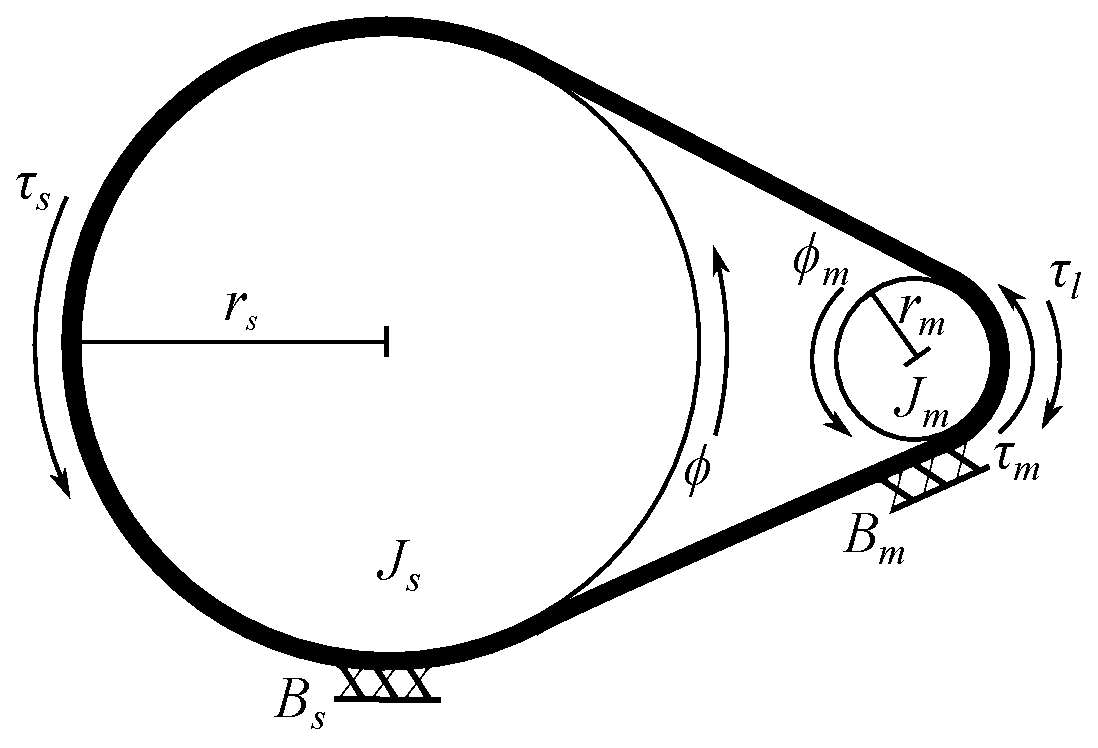
\includegraphics[width=0.80\textwidth]{figures/technical/antennaStandGearing}
	\caption{Illustration of the gearing between the DC motor and the antenna stand as a mechanical system. The spring effect of the belt strap is ignored.}
	\label{fig:antennaStandGearing}
\end{figure}

To model the antenna stands movement in respect to the voltage across the DC motor, a differential equation describing the stands movement is constructed as in \autoref{eq:standDiffEquation}.
\begin{equation} \label{eq:standDiffEquation}
J_s \cdot \frac{d \omega_{s}(t)}{d t} = \tau_{s}(t) - B_s \cdot \omega_{s}(t) \addunit{\newton\metre}
\end{equation}
\startexplain
\explain{$\tau_s(t)$ is the torque applied to the antenna stand in the azimuth plane}{\si{\newton\metre}}
\explain{$\omega_s(t)$ is the rotational speed of the antenna stand}{\si{\radian\per\second}}
\explain{$J_s$ is moment of inertia of the azimuth rotational body of the antenna stand}{\si{\newton\metre\second\squared\per\radian}}
\explain{$B_s$ is the antenna stands dampening constant}{\si{\newton\metre\second\per\radian}}
\stopexplain

Since the spring effect is assumed to be negligible, \autoref{eq:standGearingEquation} expressing the relationship between the different angular velocities and torques of the system can be derived.
\begin{equation} \label{eq:standGearingEquation}
\frac{r_s}{r_m}=\frac{\tau_s(t)}{\tau_l(t)} = \frac{\omega_m(t)}{\omega_s(t)} = N \addunit{1}
\end{equation}
\startexplain
\explain{$N$ is the gear ratio}{1}
\stopexplain

Combining \autoref{eq:standDiffEquation} and \autoref{eq:standGearingEquation} yields \autoref{eq:standDiffEquationDone}.
\begin{equation} \label{eq:standDiffEquationDone}
J_s \cdot \frac{d \omega_{s}(t)}{d t} =\tau_l(t) \cdot N - B_s \cdot \omega_{s}(t) \addunit{\newton\metre}
\end{equation}

An expression that descries the relationship between the angular velocity of the stand in respect to the current in the motor is wanted, this is archived by combining \autoref{eq:DC-motorElecEq} and \autoref{eq:DC-motorMechEqKt} with \autoref{eq:standGearingEquation}, which yields \autoref{eq:DC-motorElecDone} and \autoref{eq:DC-motorMechDone}
\begin{subequations}
	\begin{align}
	v_{s}(t) = R_{a}\cdot i_a(t) + \frac{d i_a(t)}{d t}\cdot L_a + K_{e}\cdot\omega_{s}(t)\cdot N \addunit{\volt} \label{eq:DC-motorElecDone}\\ 
	J_m \cdot \frac{d \omega_{s}(t)}{d t}\cdot N = K_t\cdot i_a(t)- \tau_l(t) - B_m \cdot \omega_{s}(t)\cdot N \addunit{\newton\metre} \label{eq:DC-motorMechDone}
	\end{align}
\end{subequations}

To determine the gear ratio for the gearing between the drive gear from the DC motor and the driven gear on the stand, the teeth of the gears are counted. The gear ratio is given by \autoref{eq:CountYourWayToAGearRatio}. 
\begin{equation} \label{eq:CountYourWayToAGearRatio}
N = \frac{n_s}{n_m} = \frac{130}{28} = 4.643 \addunit{1}
\end{equation}
\startexplain
\explain{$n_s$ is the number of teeth on the stand}{1}
\explain{$n_m$ is the number of teeth on the motor}{1}
\stopexplain

The moment of inertia $J_s$ and the damning factor $B_s$ are determined through tests covered in the test journal in \autoref{appendix:TJStandConstants}. The tests are done with the whole tracking system, as designed \autoref{pt:design}, attached to the stand, to ensure that the result is representative for the full system. The results are given in \autoref{tab:TechAnalStandConstants}. 
\begin{table}[h!]
	\centering
	\caption{Table of the constants of antenna stands azimuth rotational body.}\label{tab:TechAnalStandConstants}
	\begin{tabular}{l l l l}
		\textit{Component}		&	\textit{Symbol} &  	\textit{Value} &  \textit{Unit} \\ \rowcolor{lightGrey} \toprule
		Moment of inertia					&	$J_s$	& 0.012 			   & $\SI{}{\newton\metre\second\squared\per\radian}$ \\
		Motor friction coefficient					&	$B_s$	& 0.017 			   & $\SI{}{\newton\metre\second\per\radian}$ \\ \rowcolor{lightGrey}
		Gear ratio					&	$N$	& 4.643 			   & 1
	\end{tabular}	
\end{table}

Now that the DC motor and the azimuth rotational body of the antenna stand has been modelled and measured, the relationship between the position and the voltage across the motor is derived, for use during the design phase.

\subsection{Derivation of the azimuth angle, $\boldsymbol{\phi (t)}$, in respect to the DC motor supply voltage, $\boldsymbol{v_s(t)}$}\label{sec:techAnalTransferFunction}
By laplace transforming the three differential equations, \autoref{eq:standDiffEquationDone}, \autoref{eq:DC-motorElecDone} and \autoref{eq:DC-motorMechDone}, becomes Equation \ref{eq:DCMotorLaplaceStand} through c, assuming all initial variables equal zero.
\begin{subequations}
	\begin{align}
J_s\cdot \Phi (s)\cdot s^2&= N \cdot \Tau_l(s)-B_s \cdot \Phi (s) \cdot  s \label{eq:DCMotorLaplaceStand}\\
J_m\cdot \Phi (s)\cdot N\cdot s^2&=K_t \cdot I_a(s) - \Tau_l(s)-B_m \cdot \Phi (s)\cdot N \cdot  s  \label{eq:DCMotorLaplaceMotor}\\
V_s(s)&= K_e\cdot N \cdot \Phi (s)\cdot s + L_a\cdot I_a(s)\cdot s + R_a\cdot I_a(s) \label{eq:DCMotorLaplaceElectrical}
	\end{align}
\end{subequations}

Isolating $\Tau_l(s)$ in \autoref{eq:DCMotorLaplaceStand} and combining it with \autoref{eq:DCMotorLaplaceMotor} yields \autoref{eq:DCMotorFullMechanical}.
\begin{equation} 
\left( J_m\cdot N^2 + J_s\right)\cdot \Phi (s)\cdot s^2 = K_t\cdot I_a(s)\cdot N -\left( B_m\cdot N^2 +B_s \right)\cdot \Phi (s)\cdot s \label{eq:DCMotorFullMechanical}
\end{equation}

Isolating the current $I_a(s)$ in \autoref{eq:DCMotorFullMechanical} and combining it with \autoref{eq:DCMotorLaplaceElectrical}, it can be derived that the transfer function $G_{\phi} (s)=\frac{\Phi (s)}{V_s(s)}$ is as stated in  \autoref{eq:DCMotorTransferFunction}.
\begin{equation} 
G_{\phi} (s)=\frac{\frac{N\cdot K_t}{J_m L_a N^2 + J_s L_a}}{s^2+ \frac{B_m L_a N^2 + J_m N^2 R_a + B_s L_a + J_s R_a}{J_m L_a N^2 +J_s L_a} s + \frac{B_m N^2 R_a + K_e K_t N^2 + B_s R_a}{J_m L_a N^2 +J_s L_a}} \frac{1}{s}\label{eq:DCMotorTransferFunction}
\end{equation}

Insertion of known values from \autoref{sec:standAzimuthModel} and \autoref{tab:TechAnalDCMotorConstants} (in \autoref{sec:DC-motorTechnicalKnowledge}) into \autoref{eq:DCMotorTransferFunction} yields \autoref{eq:DCMotorHsDone}
\begin{equation} 
G_\phi (s)=\frac{\Phi (s)}{V_s(s)}=\frac{\SI{55358.174}{}}{s^2+ \SI{15954.501}{} s +\SI{182889.04}{}} \frac{1}{s}\label{eq:DCMotorHsDone}
\end{equation}

\autoref{eq:DCMotorHsDone} is the transfer function, describing the azimuth angle of the antenna stand in relation to the input voltage of the DC motor. 

%By a test covered in \autoref{appendix:AzimuthStandModelTest}\todo[inline]{author=Robin Do a test with the antenna and everything attached, in \autoref{appendix:AzimuthStandModelTest}}, it is concluded that the model is sufficient. The motorized antenna stand utilizes a stepper motor for movement in the elevation plane. The stepper motor is analyzed in the next section.

With the analysis of the DC motor concluded the stepper motor is now analysed. 

\subsection{Analysis of the stepper motor}\label{sec:techAnalAnalOfStepMotor}
Since a stepper motor does not work in the same linear fashion as a DC motor, no transfer function is found for the stepper motor. The analysis of the stepper motor includes calculations of the step size for the stepper motor.

A stepper motor is a motor that is rotating in steps. The stepper motor is a SAIA UBD stepper motor with a step angle of \SI{7.5}{\degree} (This value is given by the datasheet of the motor and is therefore without the gearbox attached.) \citep{SAIAstep}. To test the stepper motor, an A4988 driver carrier is connected to the stepper motor for simple control of the motor. 
A closed gearbox is connected to the stepper motor with no more information. A test of the gearbox is therefore necessary to determine the gear ratio. 

Knowing that the step angle of the stepper motor is \SI{7.5}{\degree}, the steps for a \SI{90}{\degree} rotation of the stepper motor are given by \autoref{Eq:switchfreq}.
\begin{equation}\label{Eq:switchfreq}
n=\frac{\Delta\theta}{\theta_{sng}} = \frac{\SI{90}{\degree}}{\SI{7.5}{\degree}~\text{step}^{-1}} = 12~\text{step}
\end{equation}
\startexplain
\explain{$n$ is number of steps needed to change the angle $\Delta\theta$ degrees}{step(s)}
\explain{$\Delta\theta$ is change in elevation angle}{\si{\degree}}
\explain{$\theta_{sng}$ is is the step size of the stepper motor without gearing}{\si{\degree}~step$^{-1}$}
\stopexplain

%It is confirmed through a test that the stepper motor rotates \SI{90}{\degree} in 12 steps. When the closed gearbox is connected to the stepper motor, it is again tested how many steps are needed for a \SI{90}{\degree} rotation with the gearbox attached. The result of the test is that 600 steps is needed to get \SI{90}{\degree} rotation with the gearbox. The gear ratio of the gearbox is given by \autoref{eq:techAnal:stepperGearRatio}.

Two tests of the stepper motor are carried out. For both the tests the stepper motor is controlled by the driver and a microcontroller (for out test an Arduino UNO was used). For the first test the gearbox is not attached to the motor, the needed steps to rotate the motor shaft \SI{90}{\degree} are counted. For the second test the gearbox is attached to the motor and the needed steps to rotate the motor \SI{90}{\degree} are counted again. The result of the test confirms the calculations of \autoref{Eq:switchfreq}. Furthermore, the test shows that 600 steps are needed in order to rotate the stepper motor \SI{90}{\degree} when the gearbox is attached. 

The gear ratio of the gearbox can be calculated with \autoref{eq:techAnal:stepperGearRatio}, by using the reslut of the test. 
\begin{equation}
\Delta\theta = n \cdot \theta_{sng}
 \cdot N_{s} \implies N_{s}=\frac{\Delta\theta}{n \cdot \theta_{sng}} \addunit{1}\label{eq:techAnal:stepperGearRatio}
\end{equation}
\startexplain
\explain{$N_{s}$ is gear ratio of the gearbox attached to the stepper motor}{1}
\stopexplain

By inserting the known values into \autoref{Eq:switchfreq} the gear ratio is given by \autoref{eq:techAnal:stepperGearRatio2}.
\begin{equation}
N_{s} = \frac{\SI{90}{\degree}}{\SI{600}{}~\text{steps} \cdot \SI{7.5}{\degree}~\text{step}^{-1}} = 0.02 \label{eq:techAnal:stepperGearRatio2}
\end{equation}

By using the gear ratio in  \autoref{eq:techAnal:stepperGearRatio} the step size of the stepper motor with the gearbox attached can be found, as seen in  \autoref{eq:techAnal:stepperStepSize}
\begin{equation}
\theta_{step} = \theta_{sng} \cdot N_{s} =\SI{7.5}{\degree}\cdot \si{0.02} = \SI{0.15}{\degree}~\text{step}^{-1} \label{eq:techAnal:stepperStepSize}
\end{equation}

One last thing that would prove useful in controlling the stepper motor, would be knowing duration of a step. The step time $\Delta t_{s}$ is however dependent on the frequency of the controller and is therefore left as a part of the design phase in \autoref{pt:design}.

\subsection{Conclusion of antenna stand analysis}\label{sec:ConclusionAntennaStandAnalysis}
The conclusion of the antenna stand analysis is in two parts, one for each motor. 

Firstly a model describing movement in the azimuth angle has successfully been created. It is seen that the laplace transformed angle and voltage somewhat follows the transfer function \autoref{eq:DCMotorHsDoneConclusion} (found in \autoref{sec:techAnalTransferFunction})
\begin{equation}
G_\phi (s)=\frac{\Phi (s)}{V_s(s)}=\frac{\SI{55358.174}{}}{s^2+ \SI{15954.501}{} s +\SI{182889.04}{}} \frac{1}{s}\label{eq:DCMotorHsDoneConclusion}
\end{equation}

An offset have been observed in the tests covered in Appendices \ref{appendix:TJDCMotorMomentofinertia} and \ref{appendix:TJStandConstants}, this offset is most likely due to the approximations done when determining the friction coefficients $B_s$ and $B_m$, since it was observed in Appendices \ref{appendix:TJDCMotorTorqueConstant} and \ref{appendix:TJStandConstants} that the friction coefficients $B_s$ and $B_m$ are not linear. The friction coefficients have been observed to decline with increased angular velocity, resulting in a lower than expected current draw with increasing velocity when measuring the moment of inertia. Lastly a non linearity has been observed when starting and stopping rotation. The antenna stand do not start rotating before DC voltage above $\SI{1.76}{\volt}$ is applied. These values should prove useful when designing the controller in \autoref{sec:design:DCMotorController}. The existence of this non linearity might limit the overall accuracy of the final system, since very small changes in the azimuth angle might not be possible when aiming at an almost stationary target.

Secondly the stepper motor responsible for movement in the elevation plane has been analysed. Through tests and calculations it has been found to have a step size of $\theta_{step} = \SI{0.15}{\degree}~\text{step}^{-1}$. Determining the step time $\Delta t_{s}$ and therefore speed, has been left to the design phase to determine.

With the conclusion of antenna stand analysis finished, the technical analyses is complete and the system requirements is presented in the new chapter. 